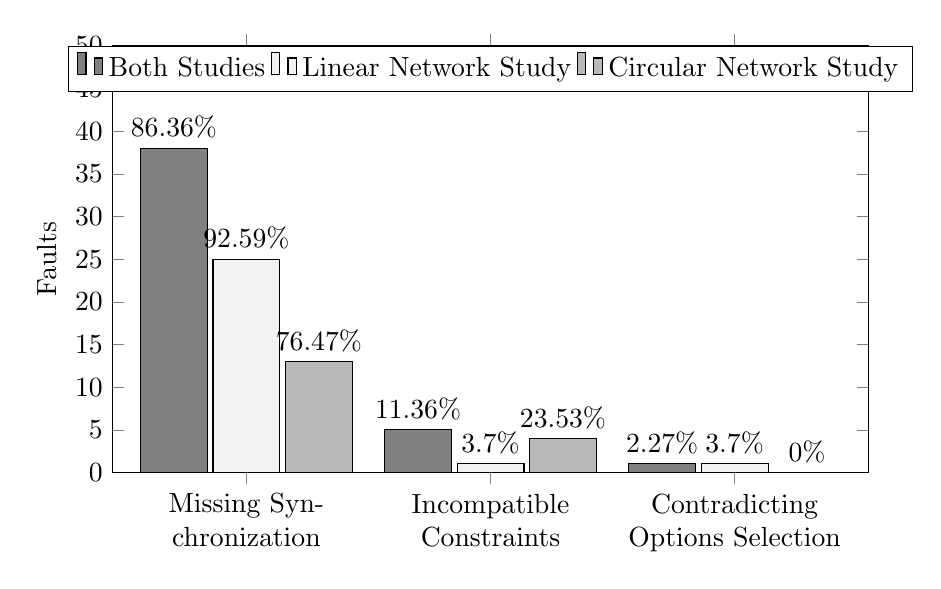
\begin{tikzpicture}
    \begin{axis}[
        ybar,
        bar width=0.85cm,
        x=3.1cm,
        height=7cm,
        legend style={at={(0.5,1)},anchor=north,legend columns=-1},
        ylabel={Faults},
        symbolic x coords={Missing Synchronization, Incompatible Constraints, Contradicting Options Selection},
        xticklabel style={text width=2.8cm, align=center},
        xtick=data,
        ytick distance=5,
        ymin=0,
        ymax=50,
        enlarge x limits={abs=1.7cm},
        nodes near coords align={vertical},
    ]
    \addplot[fill=gray,
        point meta={y*100/44}, % 44 Mistakes in total, calculate percentage
        nodes near coords={\pgfmathprintnumber\pgfplotspointmeta\%},
        ] table[x=Mistake Type, y=occurrences, col sep=comma] {
            Mistake Type,                       occurrences
            Missing Synchronization,            38
            Incompatible Constraints,           5
            Contradicting Options Selection,    1
        };
    \addplot[fill=gray!10,
        point meta={y*100/27}, % 27 Mistakes in total, calculate percentage
        nodes near coords={\pgfmathprintnumber\pgfplotspointmeta\%},
        ] table[x=Mistake Type, y=occurrences, col sep=comma] {
            Mistake Type,                       occurrences
            Missing Synchronization,            25
            Incompatible Constraints,           1
            Contradicting Options Selection,    1
        };
    \addplot[fill=gray!55,
        point meta={y*100/17}, % 17 Mistakes in total, calculate percentage
        nodes near coords={\pgfmathprintnumber\pgfplotspointmeta\%},
        ] table[x=Mistake Type, y=occurrences, col sep=comma] {
            Mistake Type,                       occurrences
            Missing Synchronization,            13
            Incompatible Constraints,           4
            Contradicting Options Selection,    0
        };
        \legend{Both Studies, Linear Network Study, Circular Network Study}
    \end{axis}
\end{tikzpicture}